\subsection*{Pangenome Analysis}
\graphicspath{{images/pangenomeAnalysis}}

% plots to be included:
% - conserved vs total genes


% Pangenome analysis:
% what’s the size of your pangenome? Is it closed or open?
% How many core and accessory genes?


Pangenome analysis found 4670 total genes (figure \ref{fig:pangenome pie}), 
among which 1017 were attributed to the \emph{core} (above 90\% prevalence in MAGs),
2074 to the \emph{shell} (from 15\% to 89\% prevalence), and 1579 were classified as \emph{cloud}
(from 0\% to 15\% prevalence). The results were robust with respect to many rounds of computation.

The number of conserved genes appears to reach a plateau (figure \ref{fig:conserved vs total}) when the number of MAGs increases, suggesting that
this species has a closed pangenome. This is further confermed by the trend of unique genes plotted against the number of genomes (figure \ref{fig:unique vs new}).




\begin{figure}[h]	% to be fixed
     \centering
     \begin{subfigure}[b]{0.4\textwidth}
         \centering
         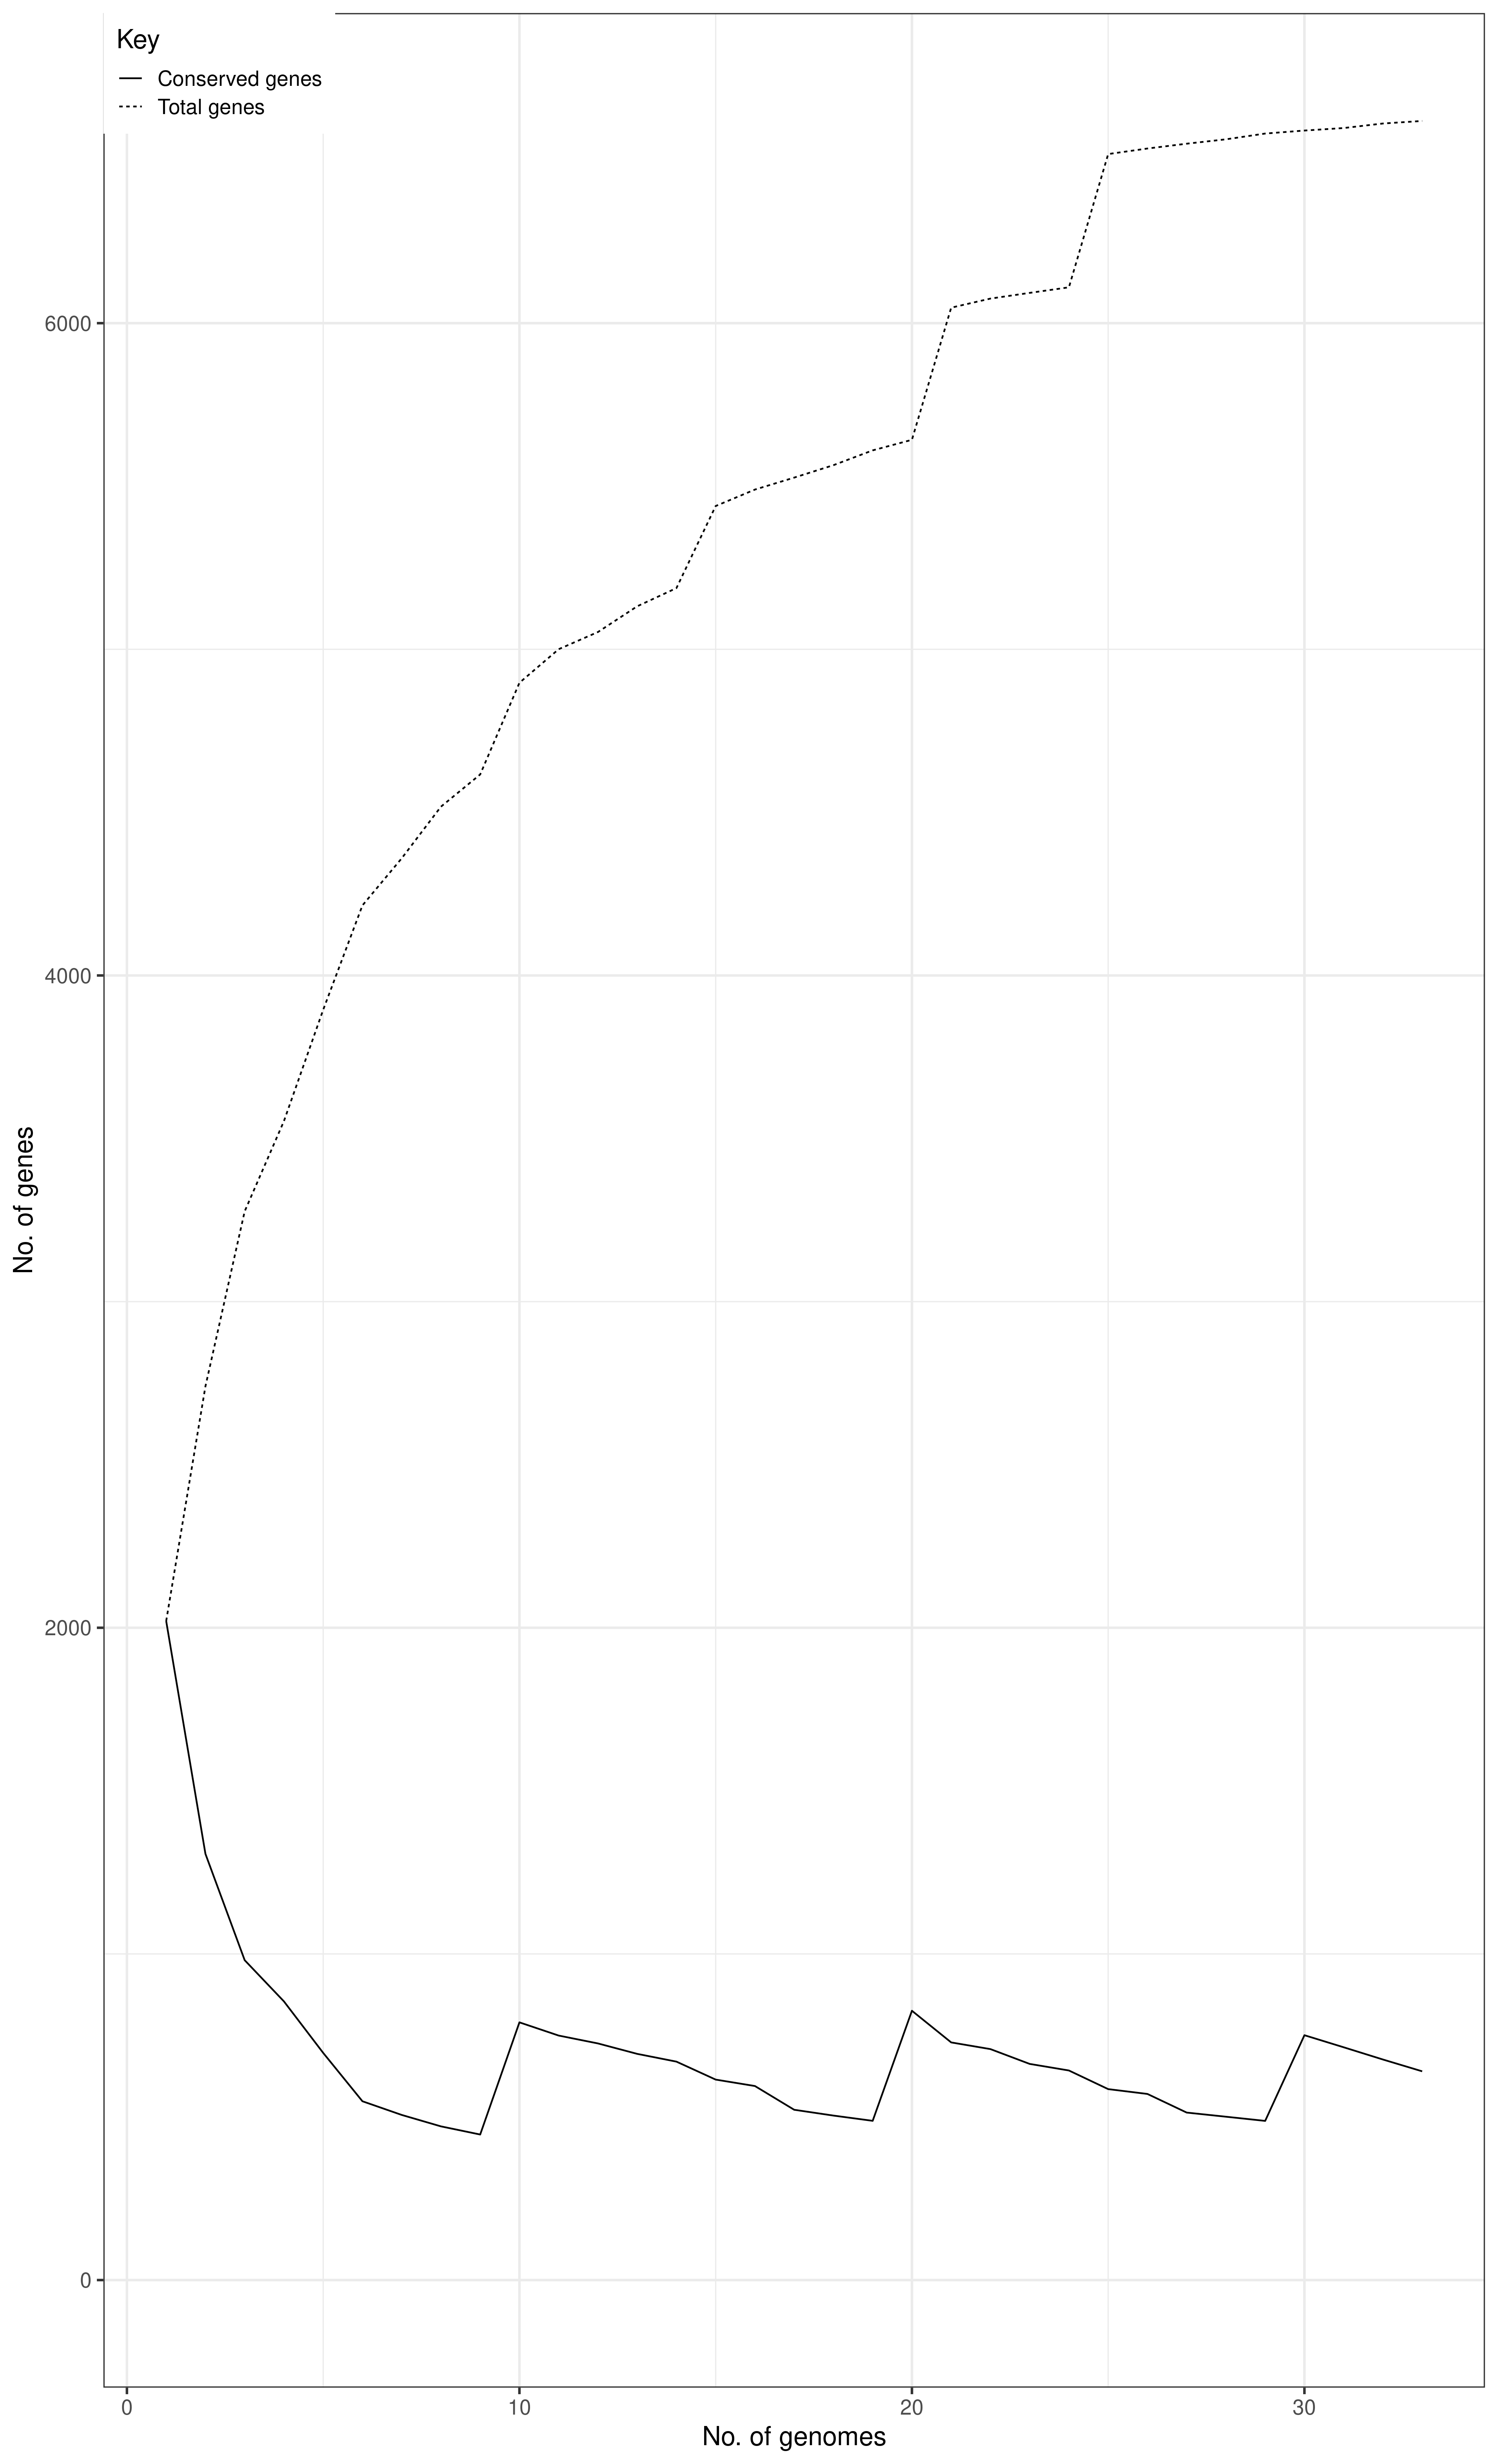
\includegraphics[width=\textwidth]{conserved_vs_total_genes}
         \caption{}
         \label{fig:conserved vs total}
     \end{subfigure}
     \hfill
     \begin{subfigure}[b]{0.4\textwidth}
         \centering
         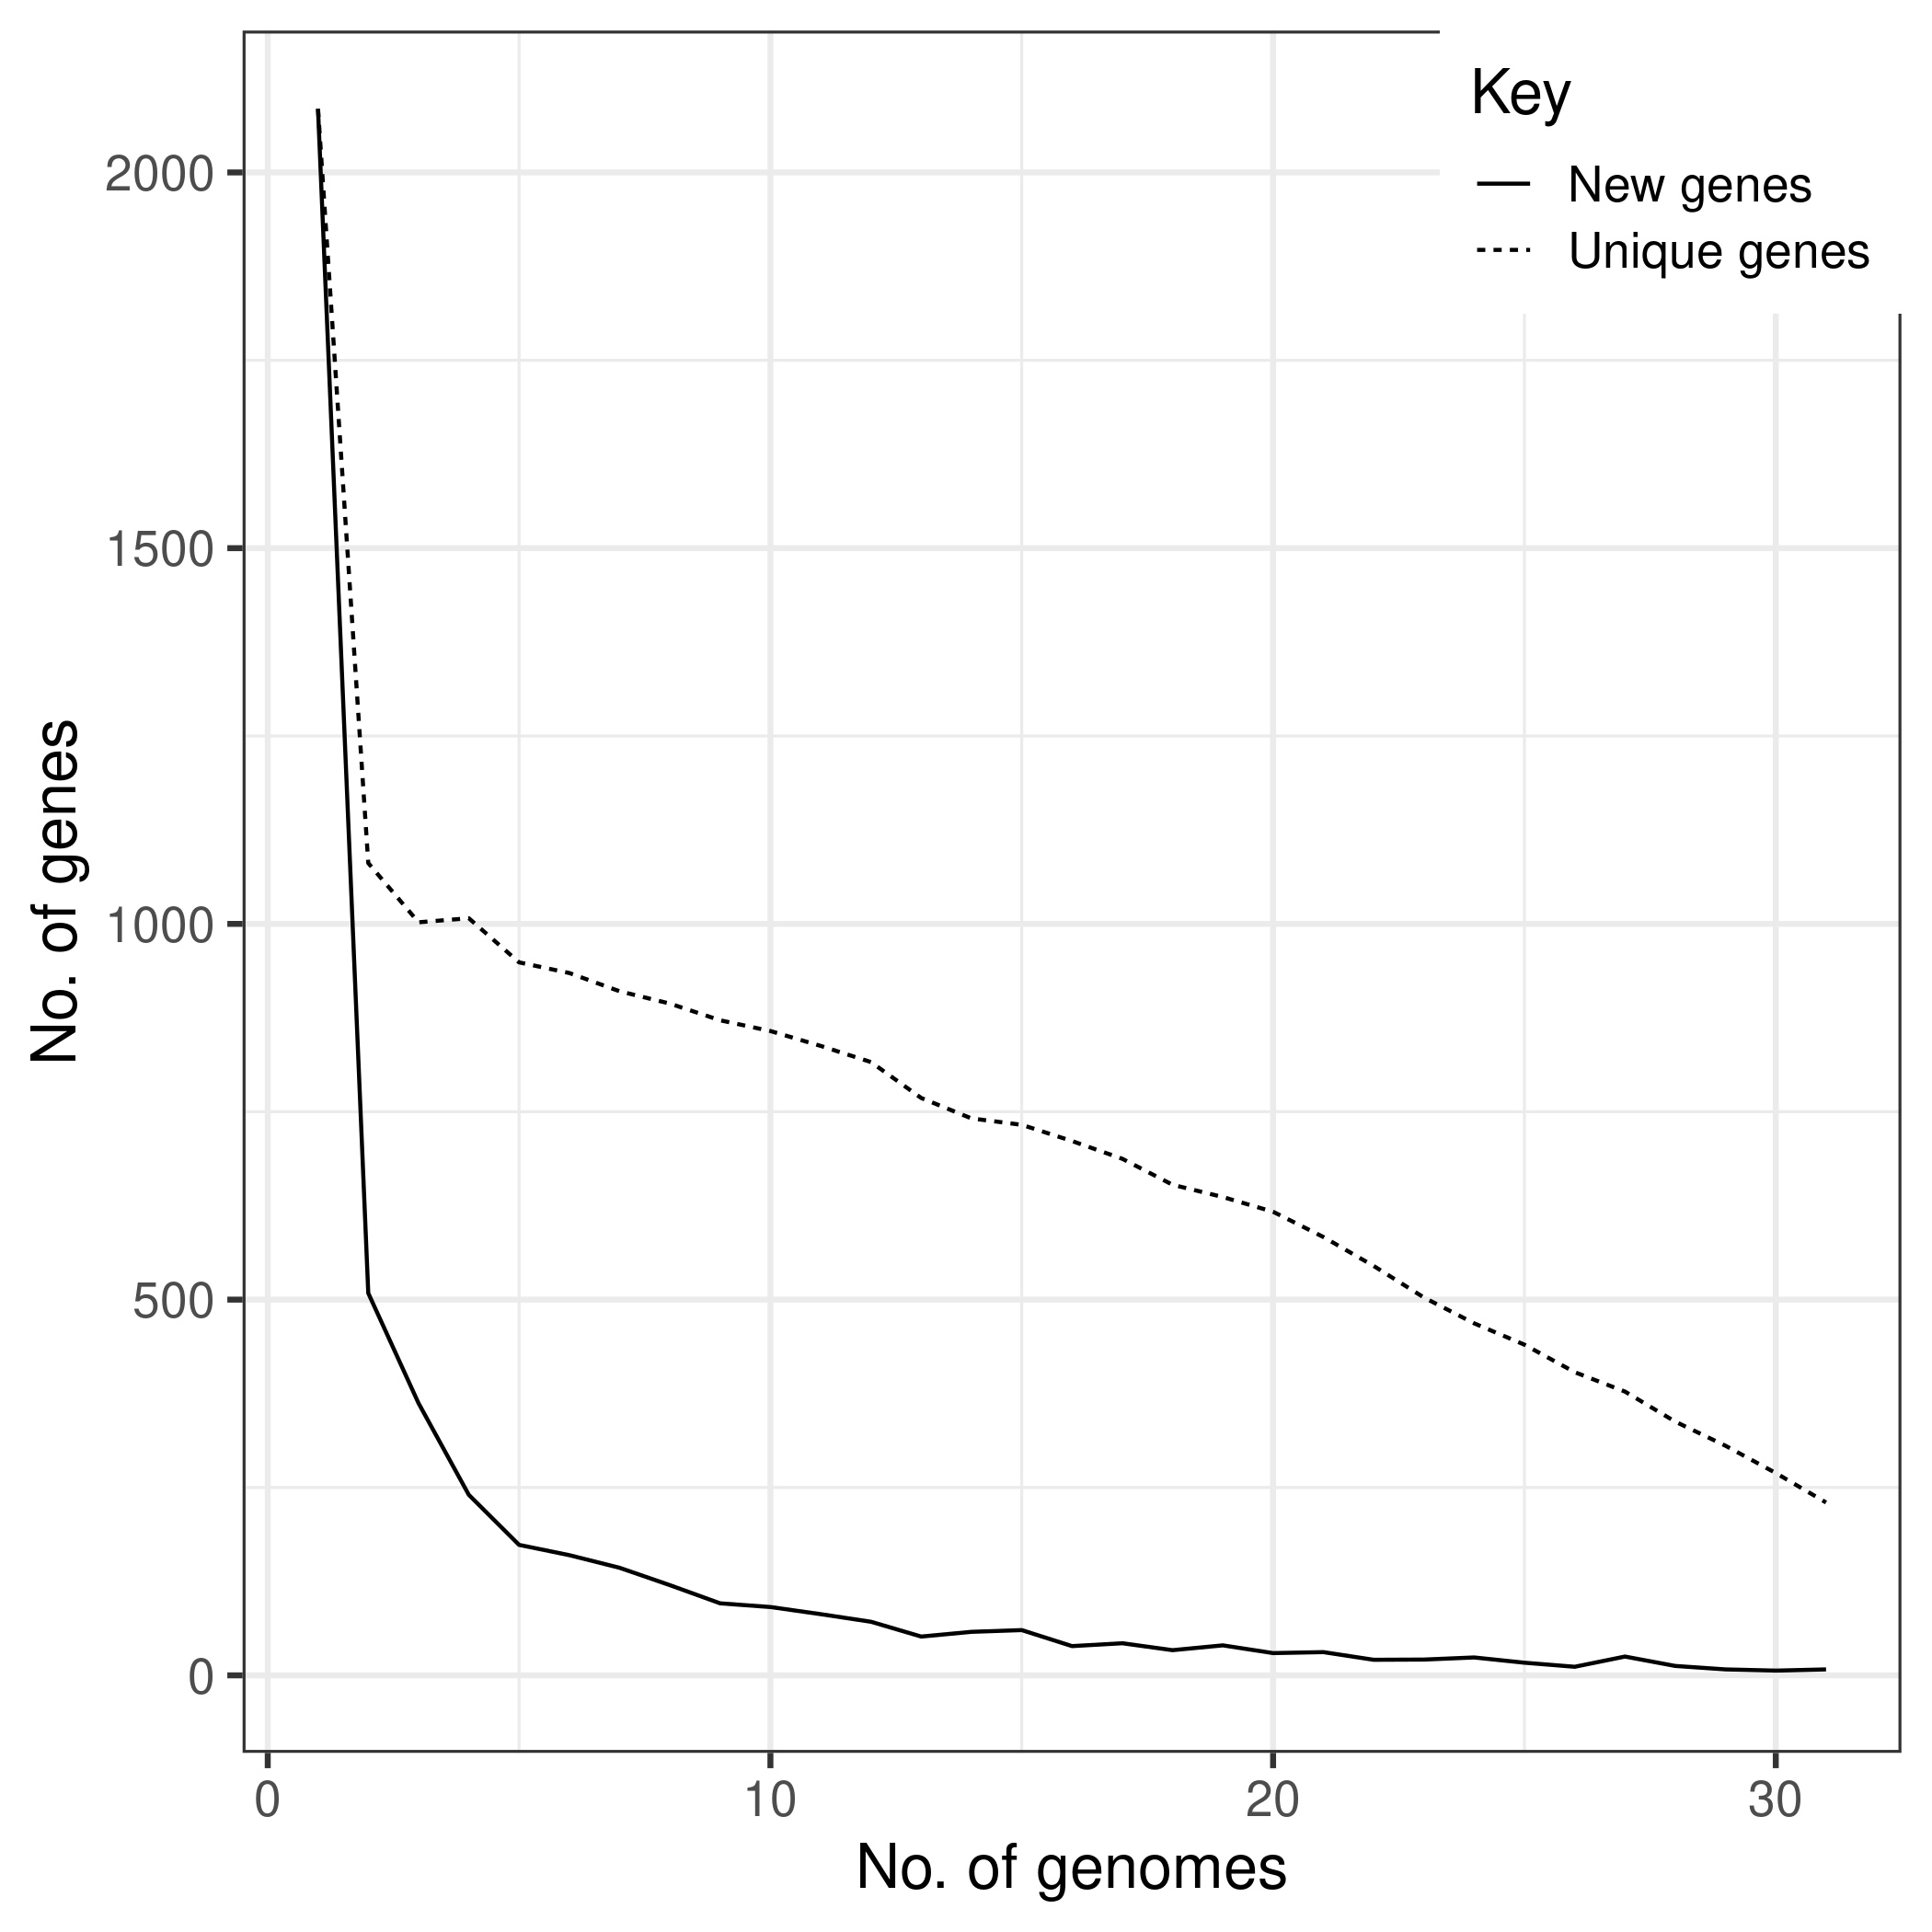
\includegraphics[width=\textwidth]{unique_vs_new_genes}
         \caption{}
         \label{fig:unique vs new}
     \end{subfigure}
        \caption{}
        \label{fig:conserved_unique_genes}
\end{figure}


\begin{figure}[h]	% to be fixed
     \centering
     \begin{subfigure}[b]{0.4\textwidth}
         \centering
         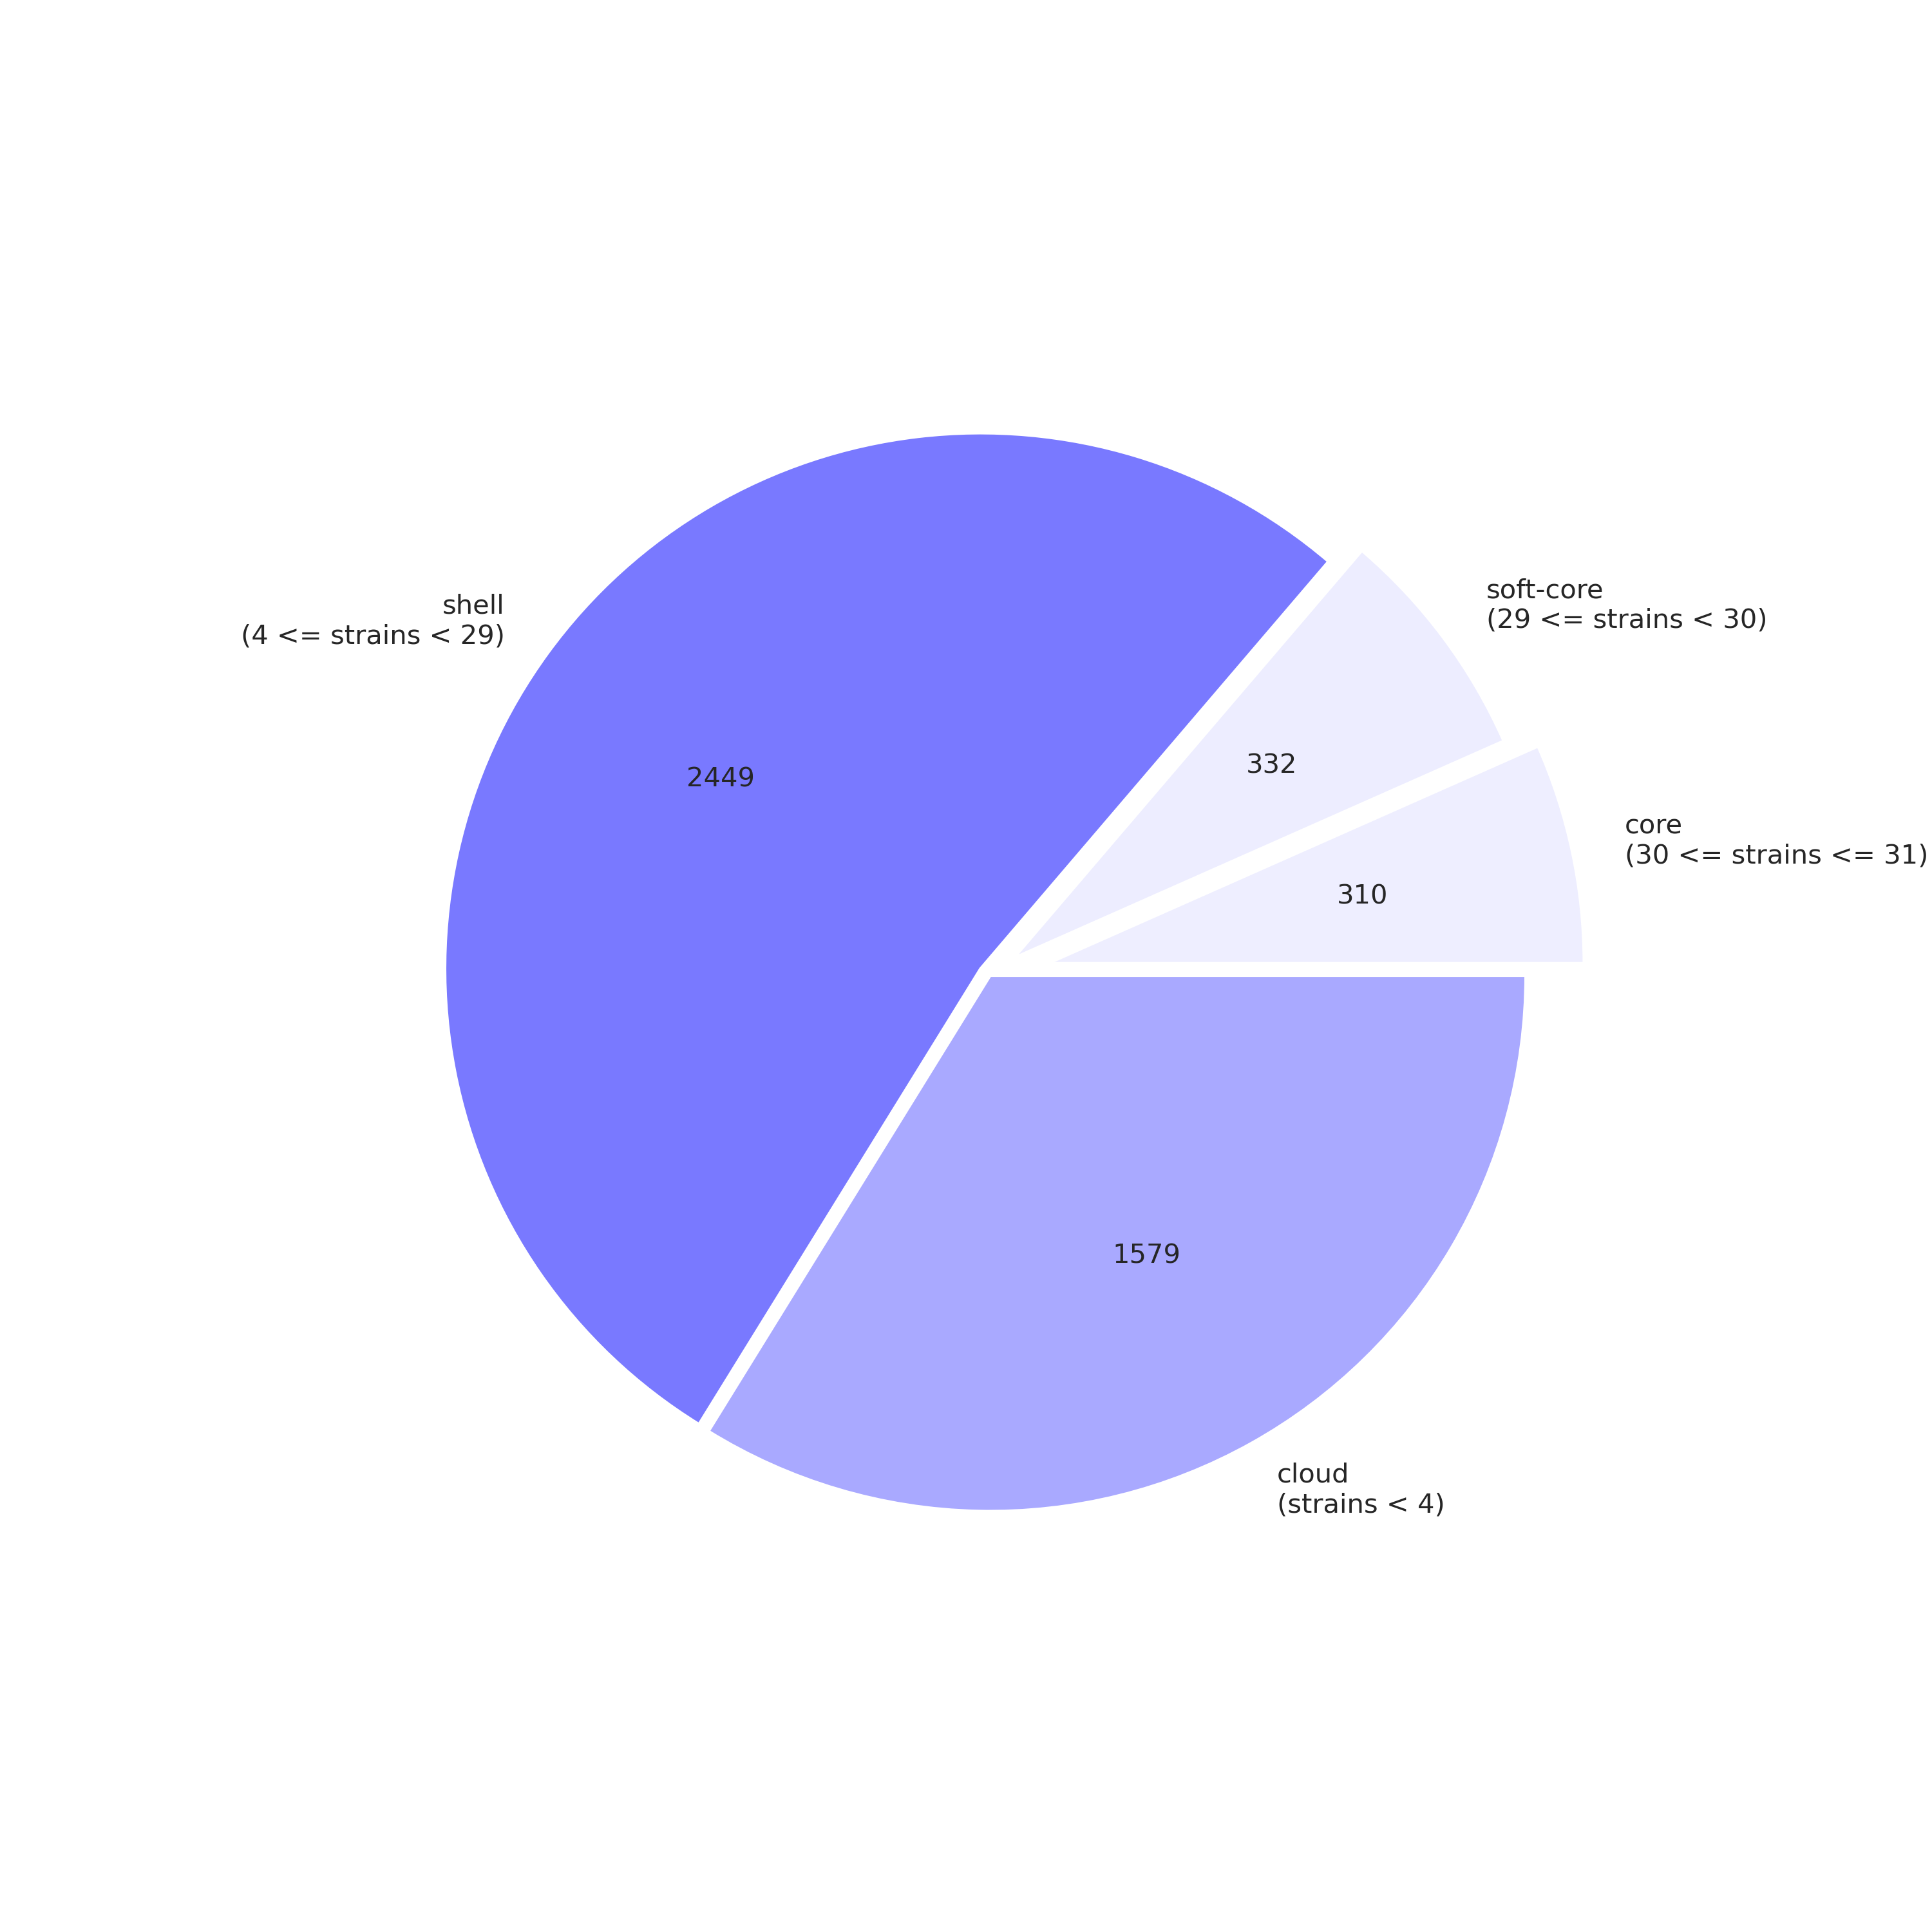
\includegraphics[width=\textwidth]{pangenome_pie}
         \caption{}
         \label{fig:pangenome pie}
     \end{subfigure}
     \hfill
     \begin{subfigure}[b]{0.4\textwidth}
         \centering
         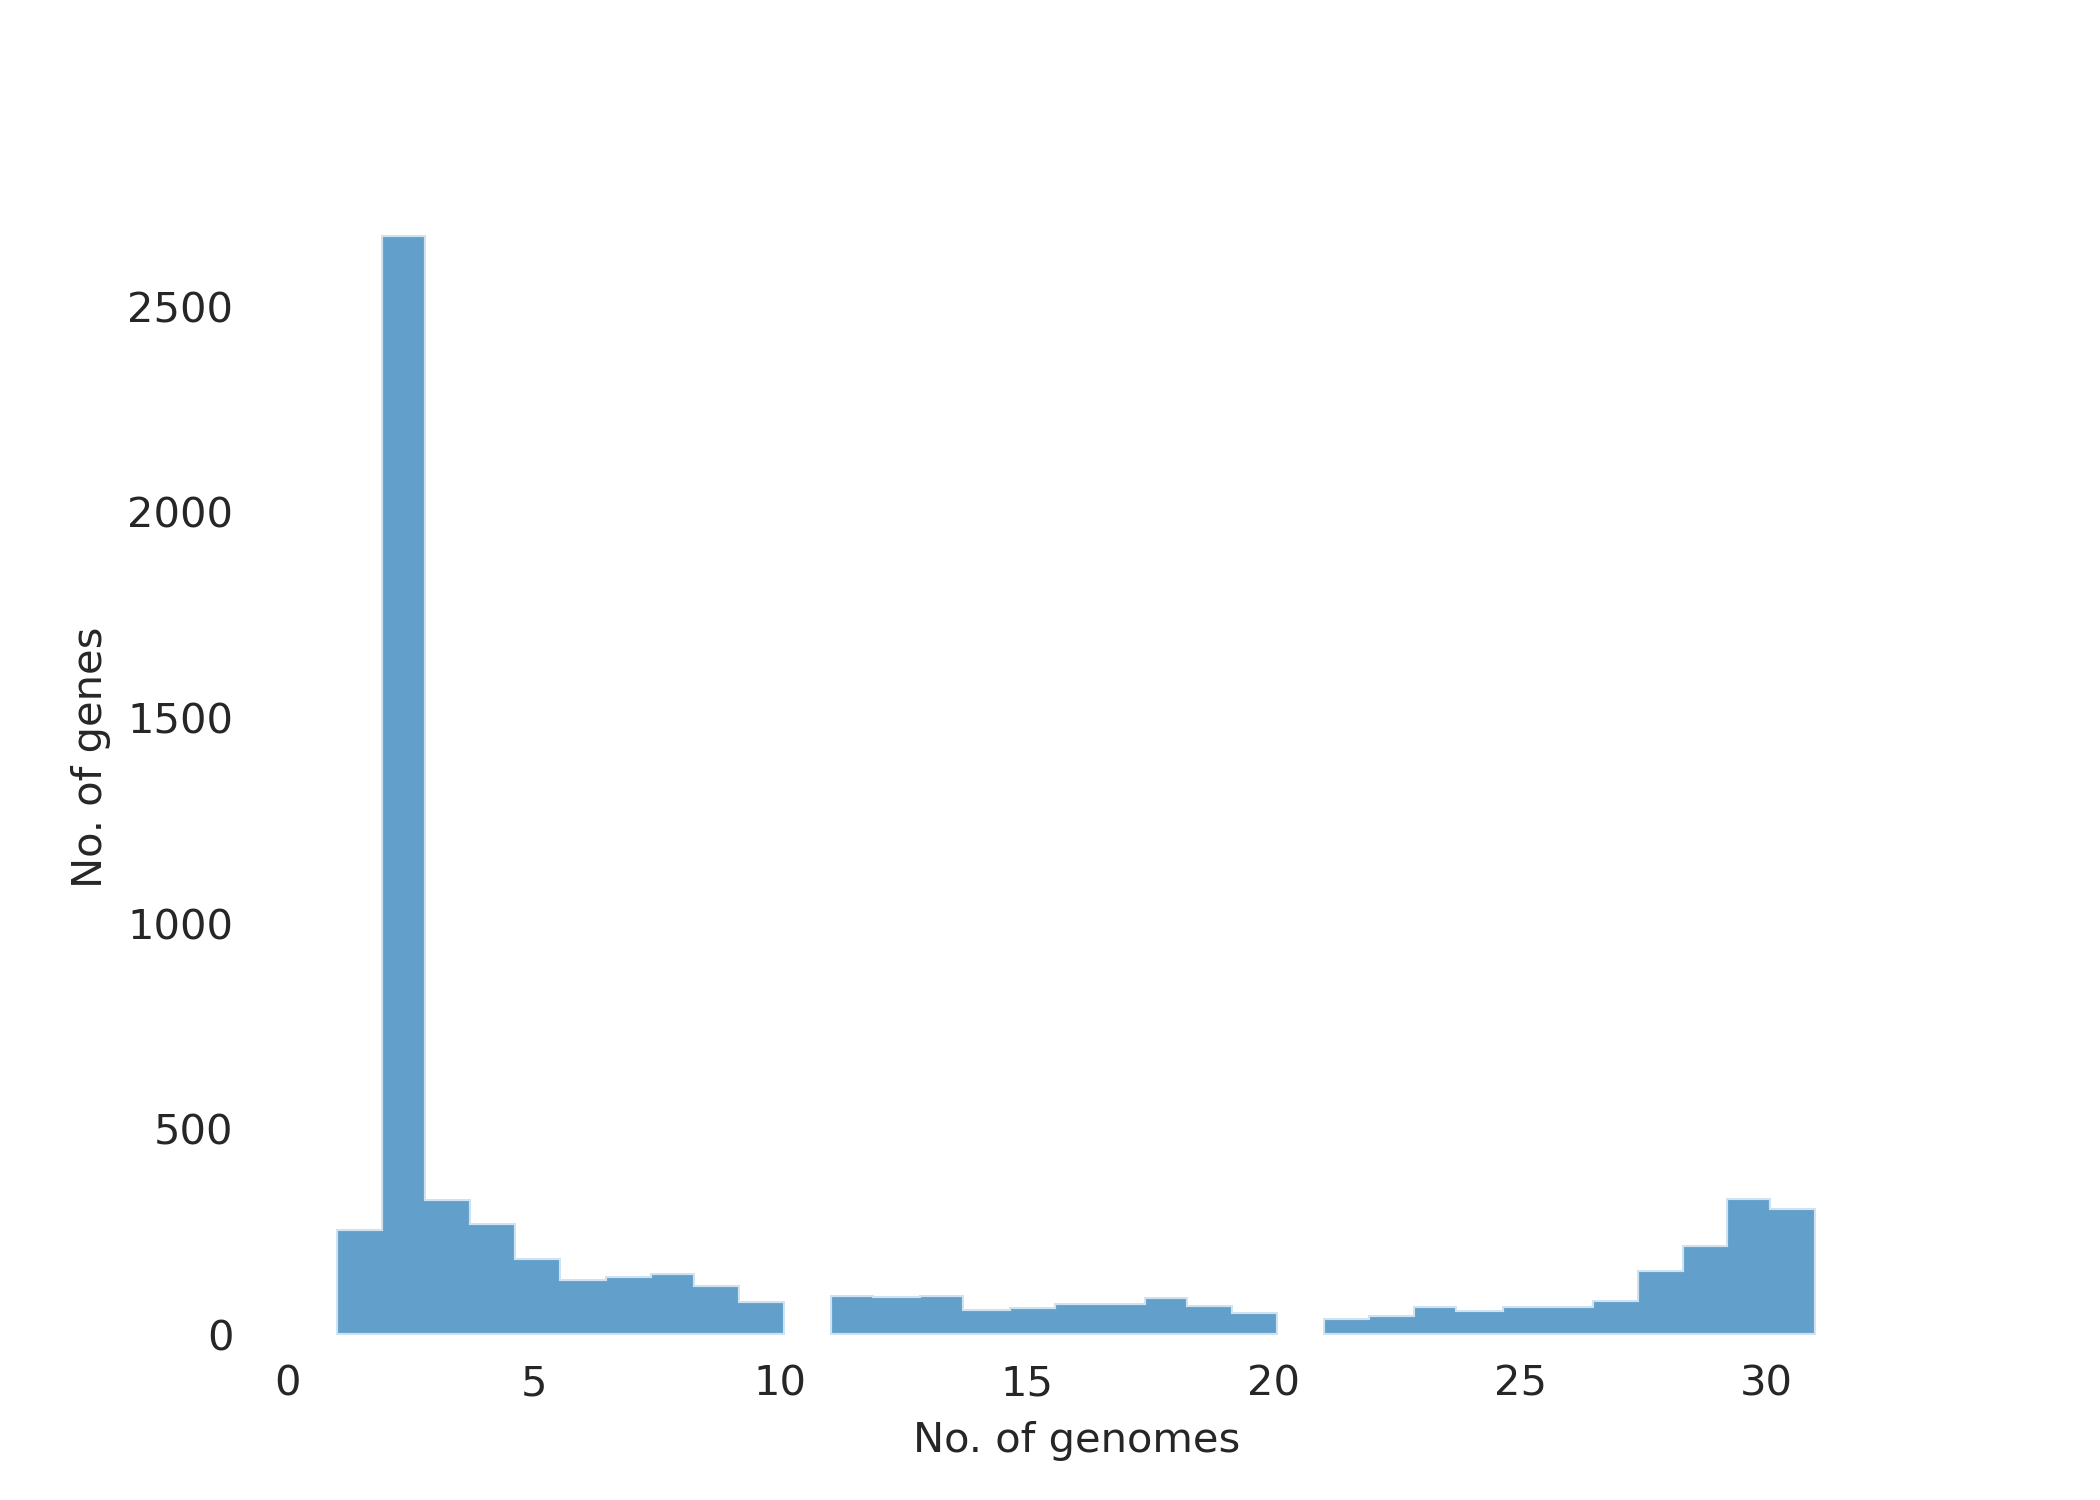
\includegraphics[width=\textwidth]{pangenome_frequency}
         \caption{}
         \label{fig:pangeome frequency}
     \end{subfigure}
     \hfill
     \begin{subfigure}[b]{0.7\textwidth}
         \centering
         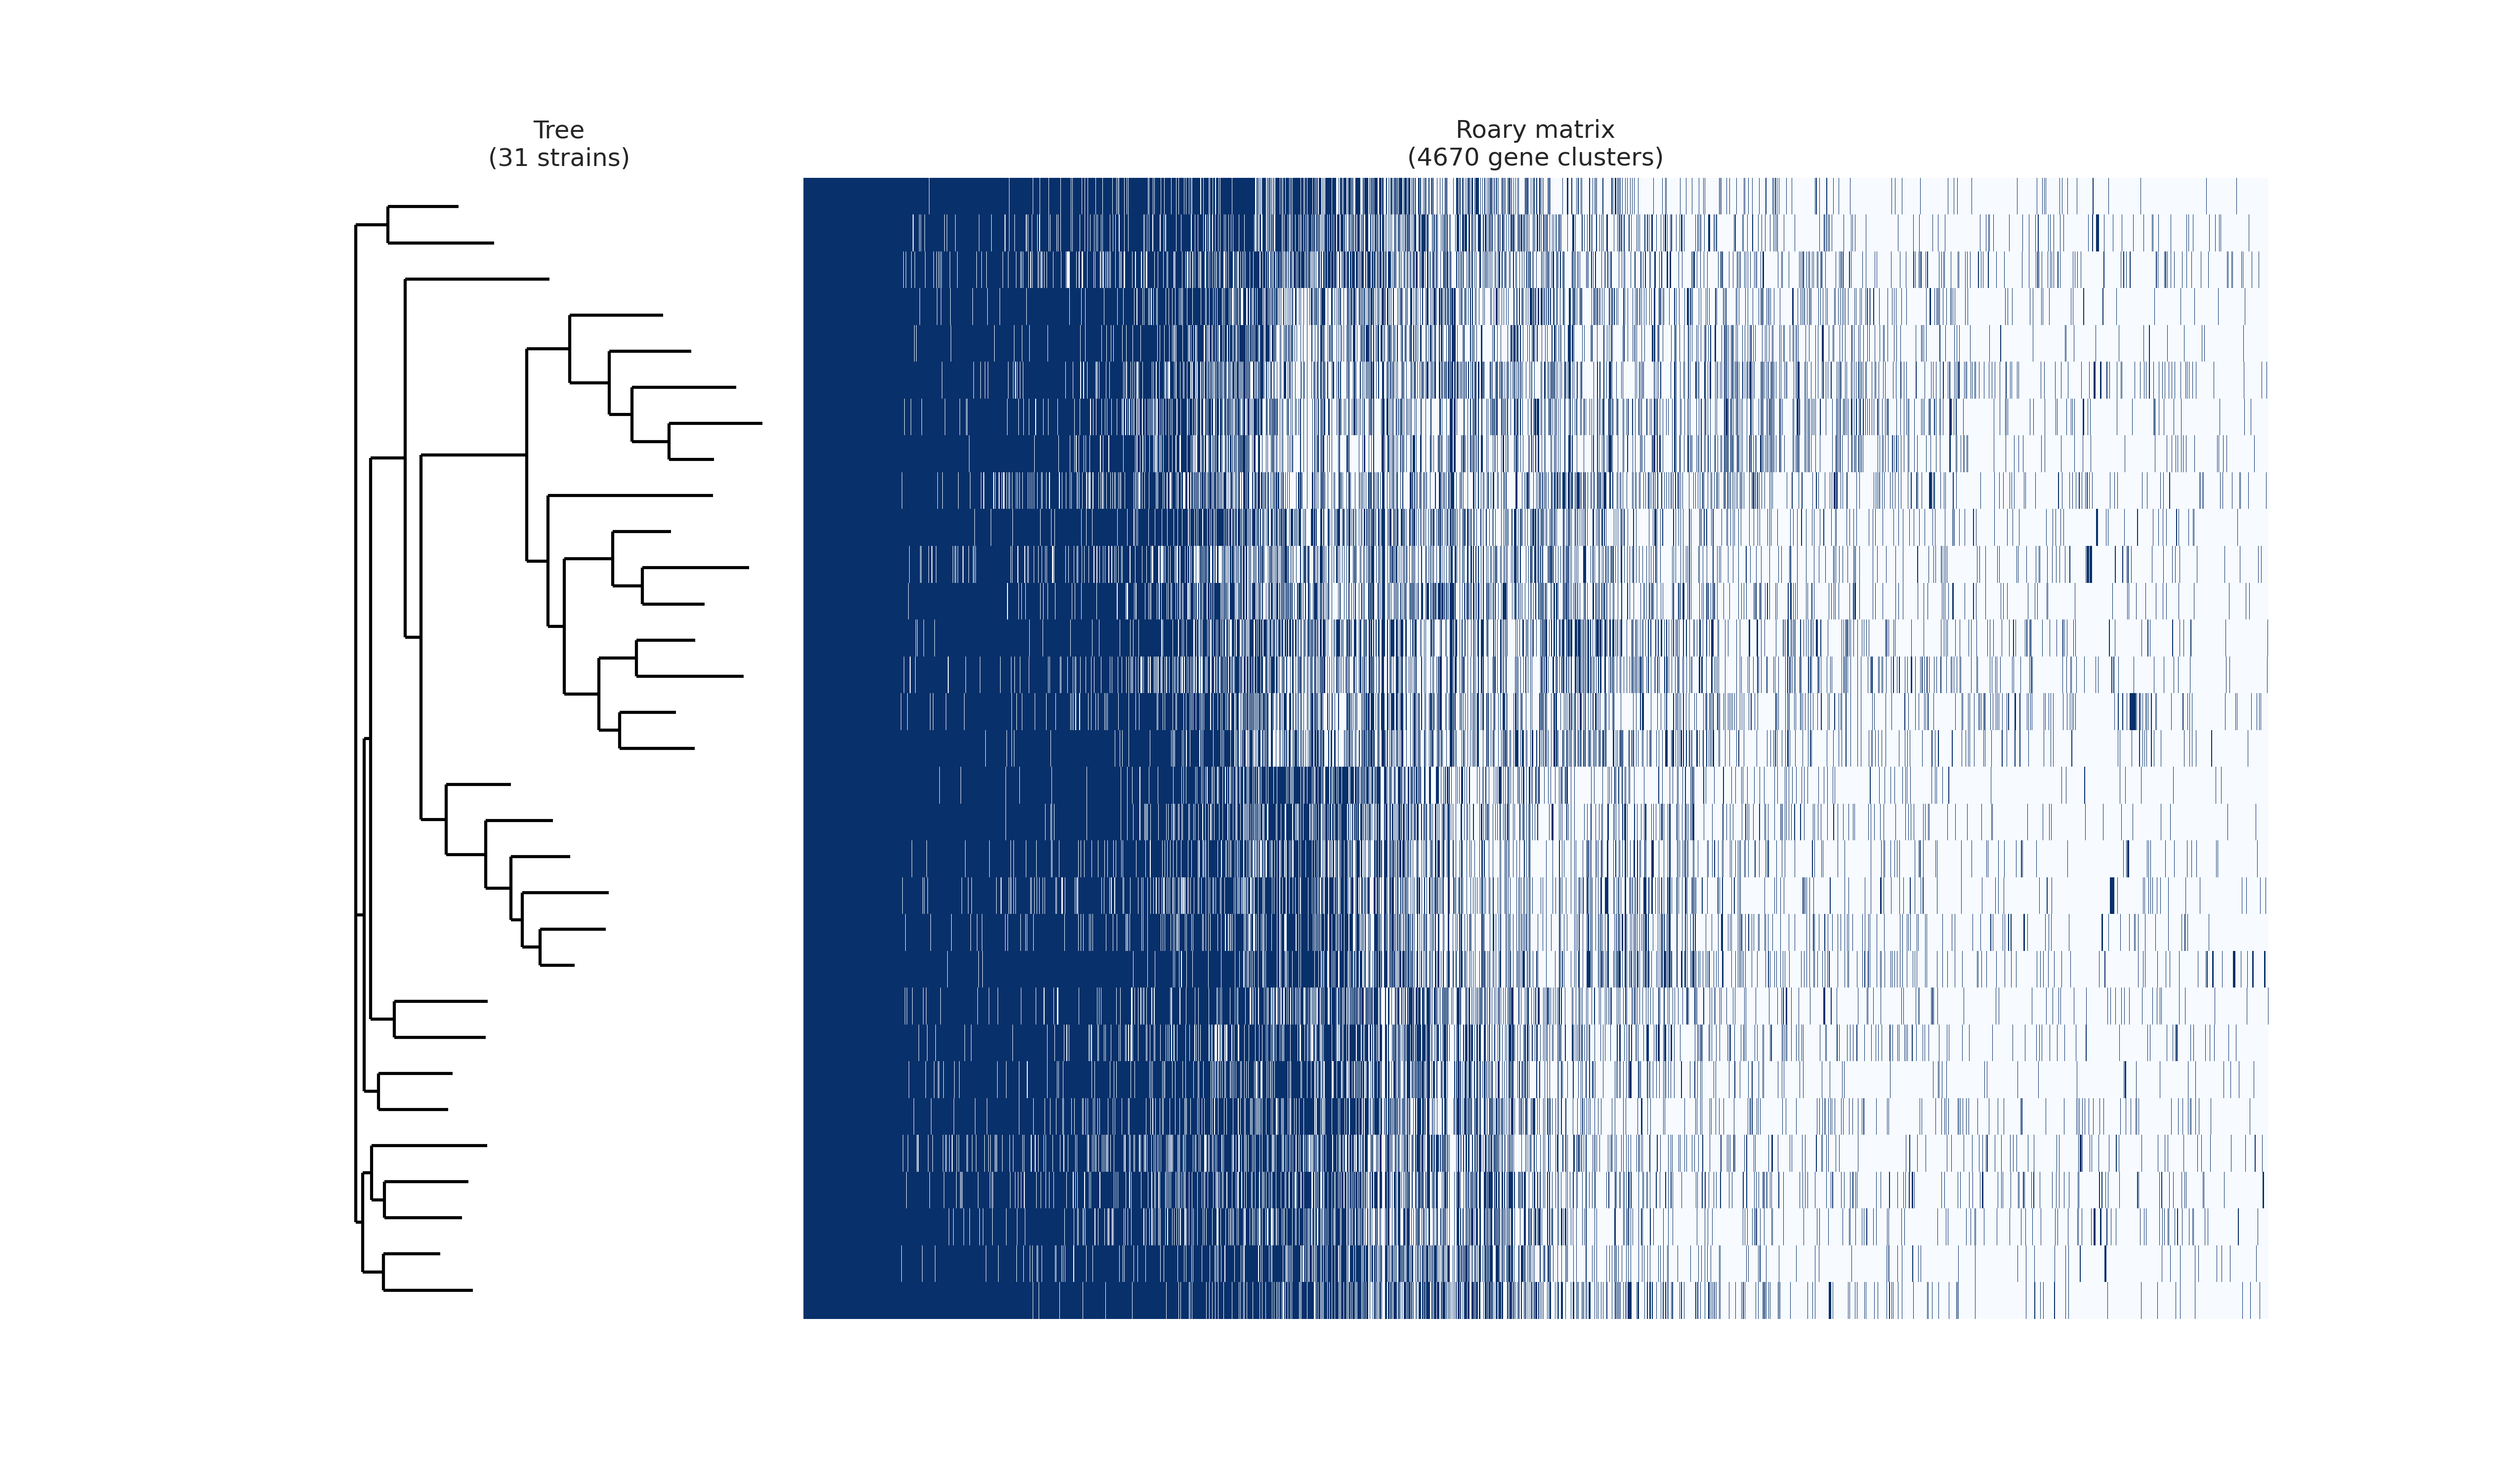
\includegraphics[width=\textwidth]{pangenome_matrix}
         \caption{}
         \label{fig:pangenome matrix}
     \end{subfigure}
        \caption{Three simple graphs}
        \label{fig:three graphs}
\end{figure}



% (https://github.com/sanger-pathogens/Roary/blob/master/bin/create_pan_genome_plots.R)
% 
% - Pangenome frequency plot
% - Presence and absence matrix and tree
% - Pangenome pie-chart (core, soft core, shell and cloud genes)
% (https://github.com/sanger-pathogens/Roary/blob/master/contrib/roary_plots/roary_plots.py)





















